\title{Warm-Up for April 6th, 2022}
\author{Dr. Jordan Hanson - Whittier College Dept. of Physics and Astronomy}
\date{\today}
\documentclass[12pt]{article}
\usepackage[a4paper, total={18cm, 27cm}]{geometry}
\usepackage{graphicx}
\usepackage{amsmath}
\usepackage{bm}
\def\rcurs{{\mbox{$\resizebox{.16in}{.08in}{
\includegraphics{ScriptR}}$}}}
\def\brcurs{{\mbox{$\resizebox{.16in}{.08in}{
\includegraphics{BoldR}}$}}}
\def\hrcurs{{\mbox{$\hat \brcurs$}}}
 
\begin{document}
\maketitle
\small
\section{Memory Bank and Review from PHYS180}
\begin{enumerate}
\item Lorentz Force, currents and charges: $\mathbf{F} = \int I d\mathbf{L} \times \mathbf{B}$ and $\mathbf{F} = q \mathbf{v} \times \mathbf{B}$
\item Work (mechanics) and centripetal force (mechanics): $W = \int \mathbf{F} \cdot d\mathbf{r}$ and $F = m r \omega^2 = mv^2/r$
\item Biot-Savart Law: 
\begin{equation}
\mathbf{B} = \frac{\mu_0}{4\pi}\int \frac{I d\mathbf{l}' \times \hat{\brcurs}}{\rcurs^2}
\end{equation}
\end{enumerate}

\section{Charge, Currents, and Magnetic Fields}

\begin{enumerate}
\item Consult the situation in Fig. \ref{fig:1}.  (a) Suppose a particle of charge $q$ with initial velocity $\mathbf{v} = 0 \hat{\mathbf{x}} + v_y \hat{\mathbf{y}}$ moves through a constant field $\mathbf{B} = B \hat{\mathbf{x}}$.  Using $\omega = 2\pi/T$, where $T$ is the period of circular motion in Fig. \ref{fig:1}, show that the charge moves in a circle with a frequency $\omega = (q/m) B$. (b) Now make the velocity $\mathbf{v} = v_x \hat{\mathbf{x}} + v_y \hat{\mathbf{y}}$ and explain the trajectory in Fig. \ref{fig:1}. (c) Does the $\mathbf{B}$-field do work on the charge $q$? \\ \vspace{2cm}
\item Using the Biot-Savart Law, show that the $\mathbf{B}$-field at the center of a circular loop of current with radius $R$ in the $xy$-plane centered at the origin is
\begin{equation}
\mathbf{B} = \frac{\mu_0 I}{2R}\hat{\mathbf{z}}
\end{equation}
\vspace{1cm}
\end{enumerate}

\begin{figure}[hb]
\centering
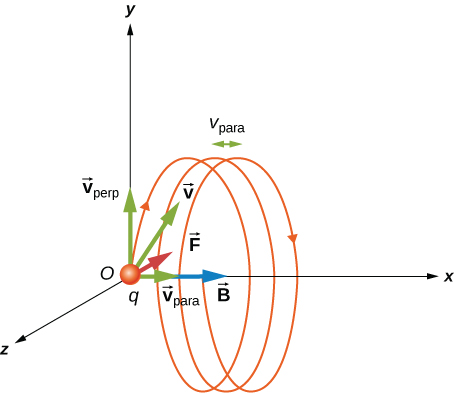
\includegraphics[width=0.3\textwidth]{figures/cyclo2.jpeg}
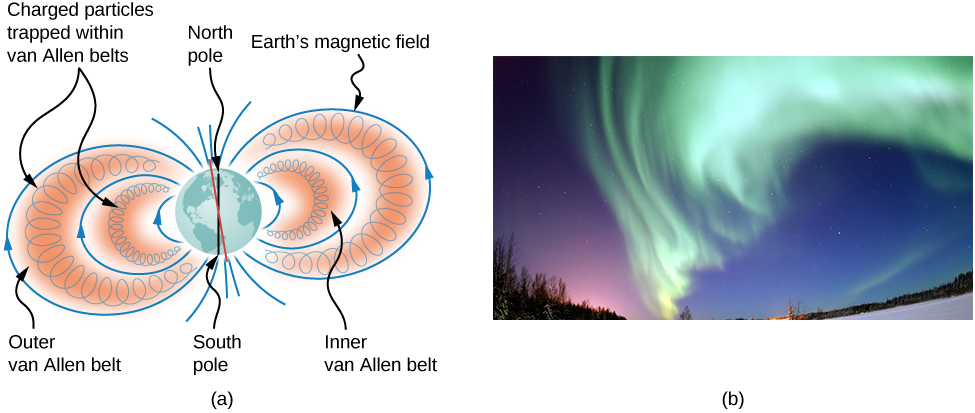
\includegraphics[width=0.3\textwidth,trim=0cm 0cm 9cm 0cm,clip=true]{figures/cyclo3.jpeg}
\caption{\label{fig:1} The aurora is caused by Solar cosmic rays interacting with the Earth's magnetic field.}
\end{figure}

\end{document}